\documentclass[aspectratio=169]{beamer}
\usepackage[utf8]{inputenc}
\usepackage{hyperref}
\usepackage{amsmath,amsfonts,amsthm,bm}
\usepackage{color}
\usepackage{graphicx} % Allows including images
\usepackage{subcaption}
\usepackage{booktabs} % Allows the use of \toprule, \midrule and \bottomrule in tables
\usepackage{tikz}
\usetikzlibrary{automata,positioning,shapes.geometric,shapes.misc,arrows}
%\usepackage{pgfplots}
\usepackage{listings}
\usepackage{courier}
\usepackage[version=4]{mhchem}
\usepackage{array}

\lstset{ %
    basicstyle=\scriptsize\ttfamily, % fonts that are used for the code
    breakatwhitespace=false,         % sets if automatic breaks should only happen at whitespace
%breaklines=true,                 % sets automatic line breaking
%captionpos=b,                    % sets the caption-position to bottom
    commentstyle=\color{gray}\textit,    % comment style
    keepspaces=true,                 % keeps spaces in text, useful for keeping indentation of code (possibly needs columns=flexible)
    keywordstyle=\color{blue},       % keyword style
    language=Python,                 % the language of the code
%otherkeywords={*,...},          % if you want to add more keywords to the set
    rulecolor=\color{black},         % if not set, the frame-color may be changed on line-breaks within not-black text (e.g. comments (green here))
    showspaces=false,                % show spaces everywhere adding particular underscores; it overrides 'showstringspaces'
    showstringspaces=false,          % underline spaces within strings only
    showtabs=false,                  % show tabs within strings adding particular underscores
    stringstyle=\color{red}, % string literal style
    tabsize=4,                       % sets default tabsize to 2 spaces
    columns=fixed                    % Using fixed column width (for e.g. nice alignment)
}

\hypersetup{
    colorlinks=true,
    linkcolor=red,
    filecolor=magenta,
    urlcolor=red,
}

\DeclareMathOperator*{\argmax}{argmax}
\DeclareMathOperator*{\argmin}{argmin}
\let \vec \mathbf

\newcommand{\classname}{NANO266}
\newcommand{\classyear}{Fall 2024}
\mode<presentation> {
    \usetheme{CambridgeUS}
    \setbeamertemplate{footline}[text line]{%
        \parbox{\linewidth}{\vspace*{-8pt}\classname\hfill\classyear\hfill\insertpagenumber}}

    %\setbeamertemplate{footline}[page number]
    \setbeamertemplate{navigation symbols}{}
}


\title[\classname Properties of Periodic Solids from QM]{\classname~- Quantum Mechanical Modeling of Materials and Nanostructures\\Properties of Periodic Solids from QM}

\author{Shyue Ping Ong}
\institute[UCSD]{University of California, San Diego\\
\medskip
}
\date{\classyear} % Date, can be changed to a custom date

\begin{document}


    \begin{frame}
        \titlepage % Print the title page as the first slide
    \end{frame}

    \begin{frame}{Typical Calculation Workflow}
        \begin{figure}
            \centering
            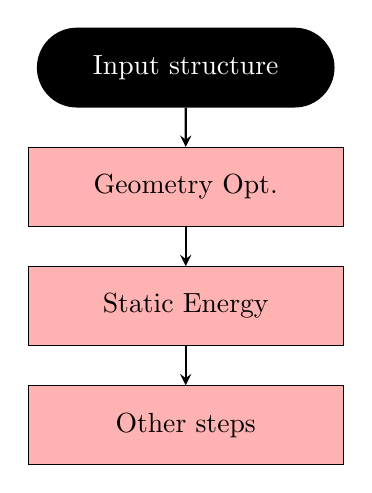
\begin{tikzpicture}[node distance=0.5cm]
                \tikzstyle{io} = [rounded rectangle, minimum width=4cm, minimum height=1cm,text centered, draw=black, fill=black, text=white]
                \tikzstyle{process} = [rectangle, minimum width=4cm, minimum height=1cm,text centered, draw=black, fill=red!30]
                \tikzstyle{decision} = [diamond,
                draw = purple,
                text = red,
                fill = pink!50,
                minimum width = 2.5cm,
                minimum height = 3cm]
                \tikzstyle{arrow} = [thick,->,>=stealth]
                \node (node1) [io, draw] {Input structure};
                \node (node2) [process, below=of node1] {Geometry Opt.};
                \node (node3) [process, below=of node2] {Static Energy};
                \node (node4) [process, below=of node3] {Other steps};

                \draw [arrow] (node1) -- (node2);
                \draw [arrow] (node2) -- (node3);
                \draw [arrow] (node3) -- (node4);
            \end{tikzpicture}
        \end{figure}

    \end{frame}

    \begin{frame}{Geometry Optimization}
        Otherwise know as ``relaxing the structure''\newline
        \newline
        Typical options in geometry optimization
        \begin{itemize}
            \item Full: cell shape, size and position of atoms are allowed to change.
            \item Fixed cell shape and size: Only position of atoms are allowed to change. E.g., defect calculations, surface calculations, etc.
            \item Constrained: Some atoms are not relaxed (useful in reducing the cost of calculations in very large cells).
            \item And many other combinations… options available depend on specific software used.
        \end{itemize}

        PWSCF: calculation=``relax'' or ``vc-relax''

        VASP: ISIF = 2 (positions only) or 3 (full)

    \end{frame}

    \begin{frame}{Manual Geometry Optimizations}
        \begin{figure}
            \centering
            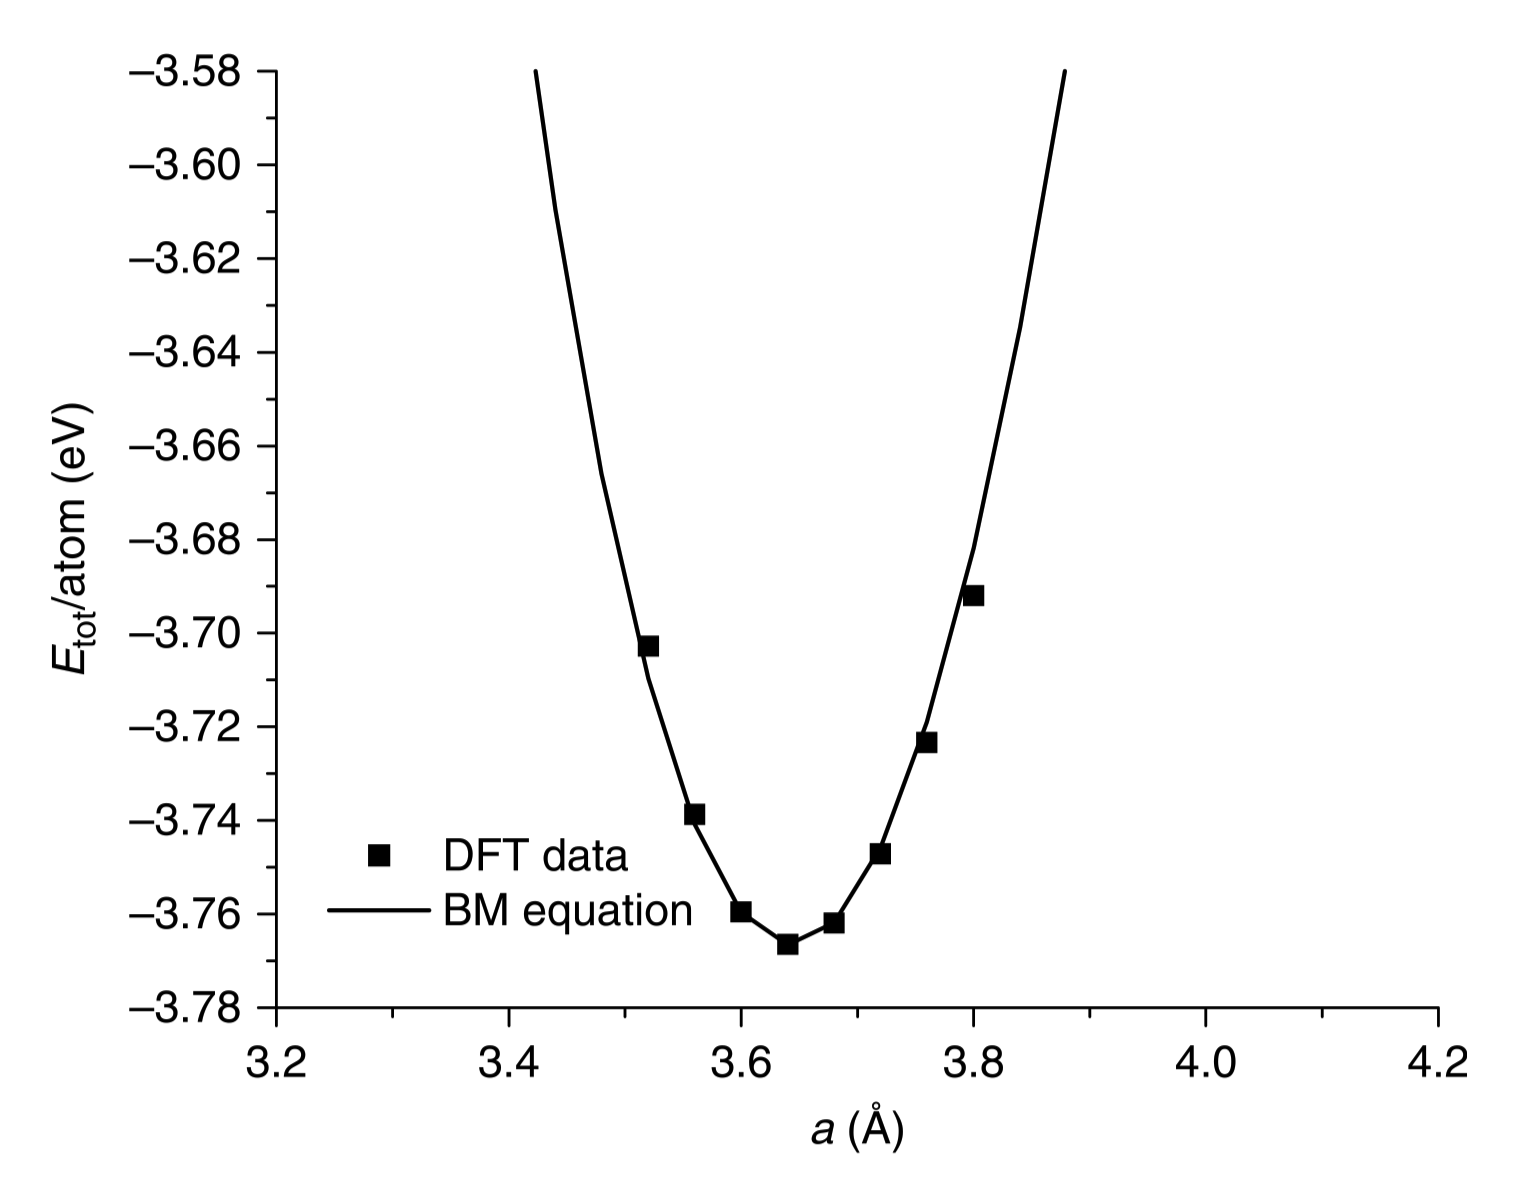
\includegraphics[width=0.45\linewidth]{lectures/figures/8_Cu_EOS.png}
            \caption{Total energy, E, of Cu in the fcc crystal structure as a function of the lattice parameter, a. Data points are from DFT calculations and the dashed curve is the Birch–Murnaghan equation of state.\cite{shollDensityFunctionalTheory2009}}
        \end{figure}
    \end{frame}


    \begin{frame}{Optimization Algorithms}

        \begin{columns}
            \column{0.6\textwidth}
            Most codes supports many options. Some common ones include:
            \begin{itemize}
                \item Quasi-newton: Newton's method for finding local minima/maxima, but with approximations for the derivatives of the functions. E.g., BFGS, FIRE, etc.
                \item Conjugate gradient: Typically requires fewer steps to reach minima.
            \end{itemize}
            \column{0.4\textwidth}
            \begin{figure}
                \centering
                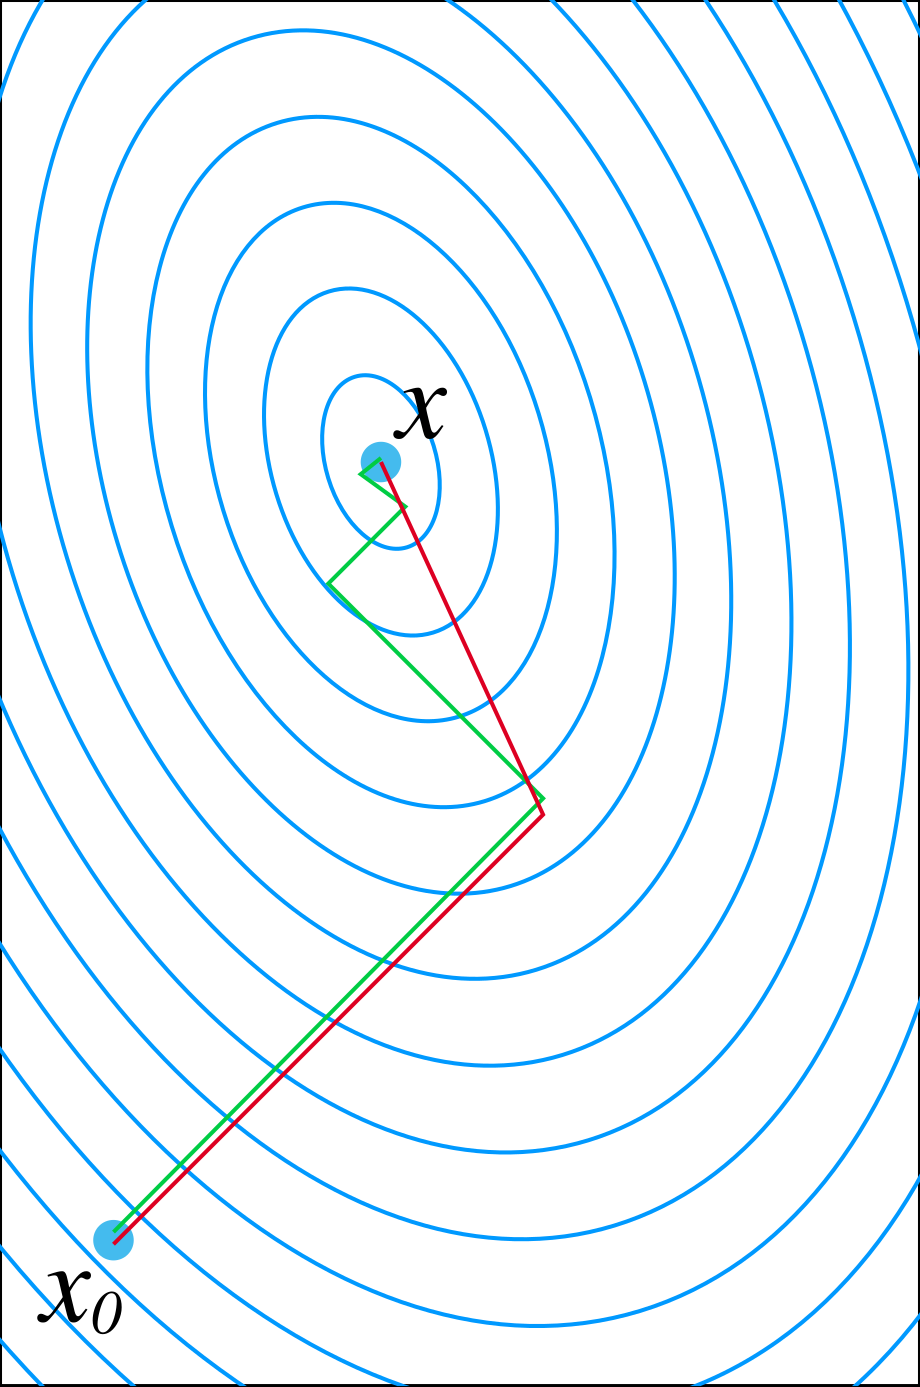
\includegraphics[width=0.5\linewidth]{lectures/figures/8_conjugate_gradient.png}
                \caption{Convergence of gradient descent (green) and conjugate gradient (red) for minimizing a quadratic function.}
            \end{figure}
        \end{columns}

    \end{frame}

    \begin{frame}{Phase transitions under pressure}

        \begin{figure}
            \centering
            \begin{subfigure}{0.45\textwidth}
                \centering
                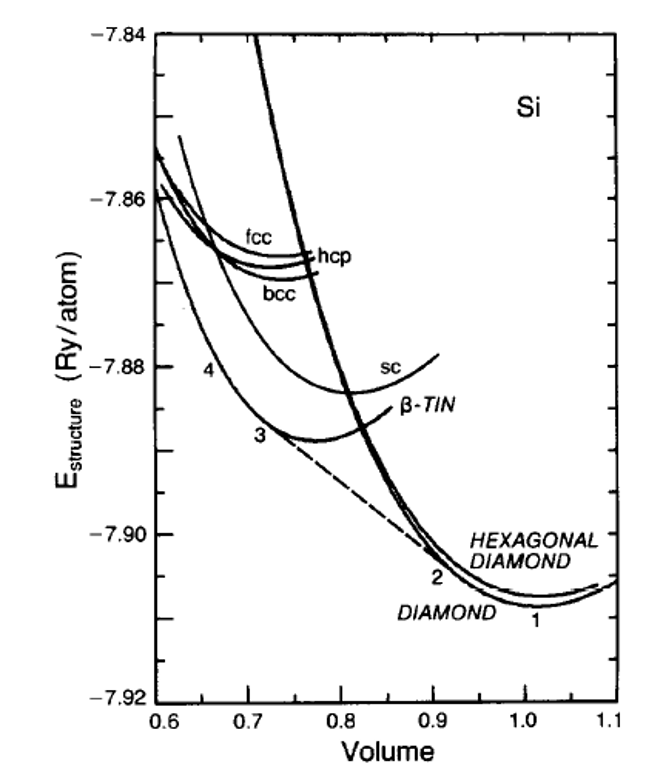
\includegraphics[width=0.7\linewidth]{lectures/figures/5_phase_diagram_si.png}
                \caption{Phase diagram of Si from LDA.\cite{yinTheoryStaticStructural1982} Transition pressure given by $P = -\frac{\partial E}{\partial V}$.}
            \end{subfigure}
            \begin{subfigure}{0.45\textwidth}
                \centering
                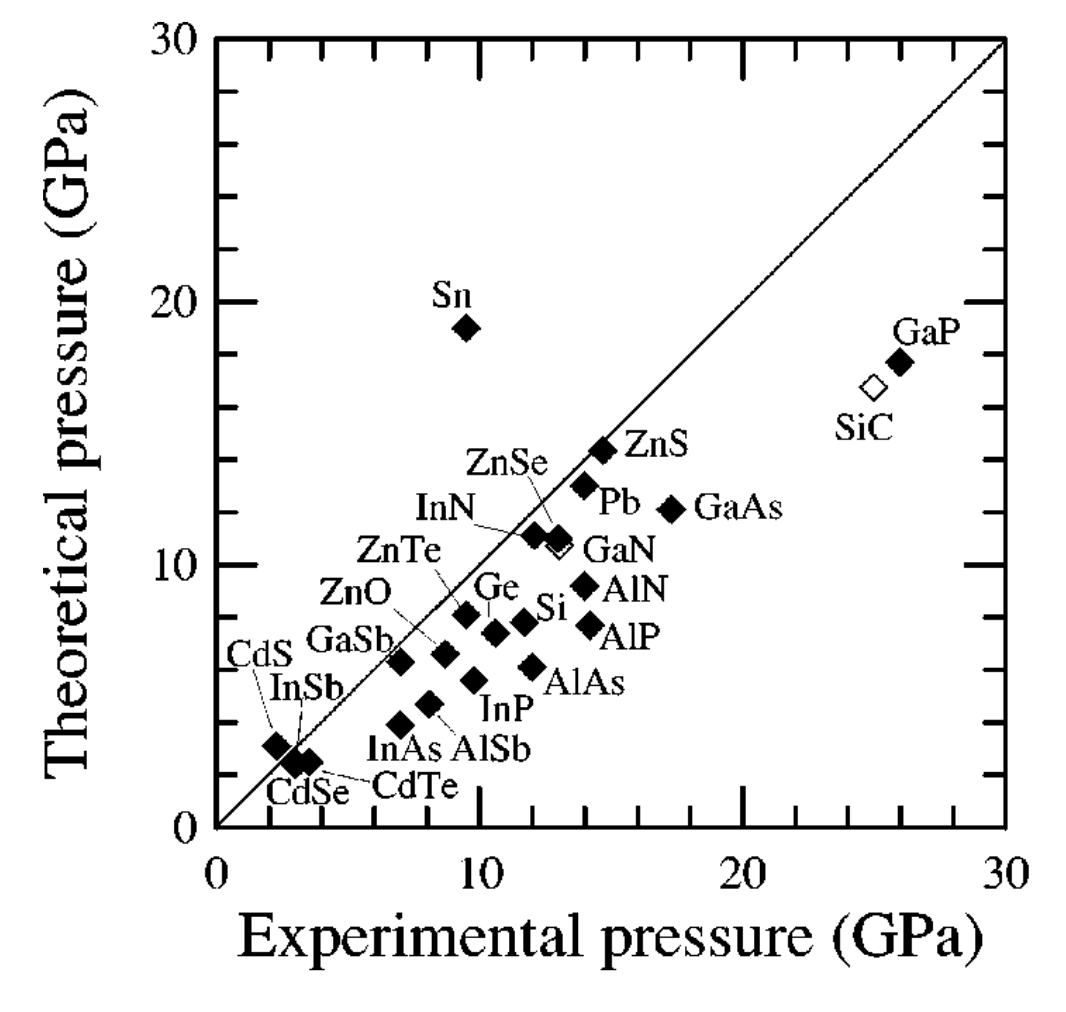
\includegraphics[width=0.8\linewidth]{lectures/figures/8_phase_transition_pressure_III_V_and_II-VI.png}
                \caption{LDA vs experimental transition pressures for the first phase transition in group-IVA elements and IIIA–VA and IIB–VIA compounds.\cite{mujicaHighpressurePhasesGroupIV2003}}
            \end{subfigure}
        \end{figure}

    \end{frame}

    \begin{frame}[allowframebreaks]{Bibliography}
        \bibliographystyle{unsrt}
        \bibliography{refs}
    \end{frame}



    \begin{frame}
        \Huge{\centerline{The End}}
    \end{frame}

\end{document}

